\documentclass{beamer}
%\usefonttheme{serif}
\usepackage{graphicx, caption}
\usepackage{subcaption}
\usepackage{amsmath,amscd, amsthm, mathrsfs, amssymb, esint}
\usepackage[utf8]{inputenc}
\usepackage{amsmath}
\usepackage{amsthm}
\usepackage{amssymb}
\usepackage{amsfonts}
\usepackage{xcolor}
\usepackage{verbatim}
\usepackage{multicol}
\usepackage{graphicx}
\usepackage{booktabs}
\usepackage{float}
\usepackage{listings}
\lstset{language=Matlab,%
    %basicstyle=\color{red},
    breaklines=true,%
    morekeywords={matlab2tikz},
    keywordstyle=\color{blue},%
    morekeywords=[2]{1}, keywordstyle=[2]{\color{black}},
    identifierstyle=\color{black},%
    stringstyle=\color{mylilas},
    commentstyle=\color{mygreen},%
    showstringspaces=false,%without this there will be a symbol in the places where there is a space
    numbers=left,%
    numberstyle={\tiny \color{black}},% size of the numbers
    numbersep=9pt, % this defines how far the numbers are from the text
    emph=[1]{for,end,break},emphstyle=[1]\color{red}, %some words to emphasise
    %emph=[2]{word1,word2}, emphstyle=[2]{style},    
}
%\usepackage{times}
%\theoremstyle{plain}
%   \newtheorem{theorem}{Theorem}[section]
%   \newtheorem{proposition}[theorem]{Proposition}
%   \newtheorem{axiom}{Axiom}
%   \newtheorem{result}{Result}
%   \newtheorem{lemma}[theorem]{Lemma}
%   \newtheorem{corollary}[theorem]{Corollary}
%   \newtheorem{conjecture}[theorem]{Conjecture}
%   \newtheorem{problem}[theorem]{Problem}
%   \newtheorem{claim}[theorem]{Claim}
%\theoremstyle{definition}
%   \newtheorem{definition}{Definition}
%   \newtheorem{technique}{Technique}
%\newtheorem{example}{Example}
%\newenvironment{solution}
%  {\begin{proof}[Solution]}
%  {\end{proof}}
% \definecolor{green}{RGB}{34, 139, 34}
 
%\pagenumbering{gobble}
 
\theoremstyle{remark}
\newcommand*{\QEDB}{\hfill\ensuremath{\square}}
\newtheorem{remark}{Remark}[section]
\renewcommand{\ss}{\mathbf{s}}
\newcommand{\BB}{\mathcal{B}}
\newcommand{\xx}{\mathbf{x}}
\newcommand{\LL}{\mathcal{L}}
\newcommand{\II}{\mathcal{I}}
\newcommand{\MM}{\mathcal{M}}
\newcommand{\yy}{\mathbf{y}}
\newcommand{\zz}{\mathbf{z}}
\newcommand{\vv}{\mathbf{v}}
\newcommand{\ww}{\mathbf{w}}
\newcommand{\NN}{\mathbb{N}}
\newcommand{\FF}{\mathcal{F}}
\newcommand{\PP}{\mathcal{P}}
\newcommand{\QQQ}{\mathcal{Q}}
\newcommand{\GG}{\mathcal{G}}
\newcommand{\PO}{\mathbb{P}}
\newcommand{\eps}{\epsilon}
\newcommand{\HH}{\mathcal{H}}
\newcommand{\quo}{\bign /}
\newcommand{\EE}{\mathcal{E}}
\newcommand{\HHH}{\overline{\mathcal{H}}}
\newcommand{\ZZ}{\mathbb{Z}}
\newcommand{\QQ}{\mathbb{Q}}
\newcommand{\RR}{\mathbb{R}}
\newcommand{\CC}{\mathbb{C}}
\newcommand{\NNN}{\mathcal{N}}
\newcommand{\CM}{\mathbb{C}_{ {MA}}}
\newcommand{\CMS}{\mathbb{C}_{ {MAS}}}
\newcommand{\sym}{\mathfrak{S}}
\newcommand{\om}{\omega}
\newcommand{\vectorthree}[3]{\begin{bmatrix} #1\\#2\\#3 \end{bmatrix}}
\newcommand{\vectortwo}[2]{\begin{bmatrix} #1\\#2 \end{bmatrix}}
\let\Vec\mathbf
\newcommand{\Cross}[2]{\Vec{#1}\times\Vec{#2}}
\newcommand{\DPartial}[2]{\frac{\partial #1}{\partial #2}}
\newcommand{\Metric}[2]{||#1 - #2||}
\newcommand{\Proj}[2]{\text{Proj}_{\Vec{#1}}(\Vec{#2})}
\newcommand{\Grad}[1]{\nabla #1}
\newcommand{\DDot}[2]{\Vec{#1}\cdot\Vec{#2}}
\newcommand{\Curl}[1]{\text{curl}\,\textbf{#1}}
\newcommand{\Div}[1]{\text{Div}\,\textbf{#1}}
\newcommand{\ps}{\text{ps}_q^1}
\renewcommand{\mod}{\mathop{\rm \ mod}}
\renewcommand{\Im}{{\rm Im}}
\renewcommand{\bar}{\overline}
\newcommand{\re}{\textbf{Re }}
\newcommand{\im}{\textbf{Im }}
\usepackage{graphics}
\usepackage{mathtools}
\usepackage[citestyle=authoryear]{biblatex}
\addbibresource{references.bib}
%\useoutertheme{miniframes} % Alternatively: miniframes, infolines, split
\useinnertheme{circles}
\definecolor{CornellRed}{RGB}{79, 0, 128} % UBC Blue (primary)
\usecolortheme[named=CornellRed]{structure}
% There are many different themes available for Beamer. A comprehensive
% list with examples is given here:
% http://deic.uab.es/~iblanes/beamer_gallery/index_by_theme.html
% You can uncomment the themes below if you would like to use a different
% one:
%\usetheme{AnnArbor}
%\usetheme{Antibes}
%\usetheme{Bergen}
%\usetheme{Berkeley}
%\usetheme{Berlin}
%\usetheme{Boadilla}
%\usetheme{boxes}
%\usetheme{CambridgeUS}
%\usetheme{Copenhagen}
%\usetheme{Darmstadt}
%\usetheme{default}
%\usetheme{Frankfurt}
%\usetheme{Goettingen}
%\usetheme{Hannover}
%\usetheme{Ilmenau}
%\usetheme{JuanLesPins}
%\usetheme{Luebeck}
%\usetheme{Madrid}
\usetheme{default}
%\usetheme{Malmoe}
%\usetheme{Marburg}
%\usetheme{Montpellier}
%\usetheme{PaloAlto}
%\usetheme{Pittsburgh}
%\usetheme{Rochester}
%\usetheme{Singapore}
%\usetheme{Szeged}
%\usetheme{Warsaw}
\usepackage{amsmath,amscd, amsthm, mathrsfs, amssymb, esint}
\usepackage{graphicx}
\usepackage{float}
\usepackage{subcaption}
%\usepackage{subfig}
\usepackage{mathtools}
%\DeclarePairedDelimiter\abs{\lvert}{\rvert}
\makeatother
\usepackage{array}
\usepackage{booktabs}
\newcommand{\lap}{\Delta}
\setbeamersize{text margin left=5mm,text margin right=5mm} 
\title{Probabilistic Quadrature Rules: From Monte Carlo to Bayes}
% A subtitle is optional and this may be deleted
\author{Shashank Sule}
% - Give the names in the same order as the appear in the paper.
% - Use the \inst{?} command only if the authors have different
%   affiliation.

\institute{Amherst College}% (optional, but mostly needed)

% - Use the \inst command only if there are several affiliations.
% - Keep it simple, no one is interested in your street address.

%\date{\today}
% - Either use conference name or its abbreviation.
% - Not really informative to the audience, more for people (including
%   yourself) who are reading the slides online

%\subject{MATH 320}
% This is only inserted into the PDF information catalog. Can be left
% out. 

% If you have a file called "university-logo-filename.xxx", where xxx
% is a graphic format that can be processed by latex or pdflatex,
% resp., then you can add a logo as follows:

% \pgfdeclareimage[height=0.5cm]{university-logo}{university-logo-filename}
% \logo{\pgfuseimage{university-logo}}

% Delete this, if you do not want the table of contents to pop up at
% the beginning of each subsection:

% \AtBeginSubsection[]
% {
%   \begin{frame}<beamer>{Outline}
%     \tableofcontents[currentsection,currentsubsection]
%   \end{frame}
% }

% Let's get started
\begin{document}

\begin{frame}
  \titlepage
\end{frame}

\begin{section}{Introduction}

\begin{frame}{Quadrature}
    \begin{itemize}
        \item How to compute
        $$ I = \int_{[0,1]}f(x)\mu(x)\,dx$$
        where $\mu$ satisfies the properties of a density function on $[0,1]$?
        \pause
        \item Example: 
        $$ I = \int_{[0,1]}x^2\,dx$$
        \pause
        $f(x) = x^2$ and $\mu(x) = \chi_{[0,1]}$
        \pause
        \item Insight: Think \textit{expected value}:
        \pause
        \begin{align}
            \mathbb{E}[f(X)] = \int_{[0,1]}f(x)\mu(x)\,dx \pause \approx \langle f \rangle = \frac{1}{N}\sum_{i=1}^{N}f(X_i)
        \end{align}
        \pause
        \item Thus, by computing the mean of $N$ independently sampled values of $f(X_i)$ we can estimate the integral $I$. This is termed \textbf{Monte Carlo} integration.
    \end{itemize}
\end{frame}
\end{section}

\begin{section}{Monte Carlo Integration}

\begin{subsection}{Simple Monte Carlo}

\begin{frame}{Monte Carlo Strategies: Simple Monte Carlo}
    \begin{itemize}
        \item Example: $f(x) = x^2$ and $\mu(x) = \chi_{[0,1]}$. \pause Then $\frac{1}{N}\sum_{i=1}^{N}x^{2}_{i} = \langle f \rangle$
        \pause
        \item Generalization: By setting $\mu(x) = \frac{1}{\text{Vol}(D)}\chi_{D}$ we can find $\int_{D}f(x)\,dx$ for any domain $D \subset \RR^n$: \pause
        $$ \int_{D}f(x)\,dx = \text{Vol}(D)\int_{D}f(x)\frac{1}{\text{Vol}(D)}\chi_{D}\,dx$$ \pause
        \item This is termed \textbf{Simple Monte Carlo}
    \end{itemize}
\end{frame}

\begin{frame}{Monte Carlo Strategies: Simple Monte Carlo}
    \begin{itemize}
        \item Let's find the volume of the 3-dimensional $L^1$ (denoted $B^{1}_{1}(0)$) unit ball using SMC!
        \pause
        $$ B^{1}_{1}(0) = \{x = (x_1, x_2, x_3) \in \RR^3 \mid |x_1| + |x_2| + |x_3| \leq 1\}$$
        \pause
        \begin{figure}
            \centering
            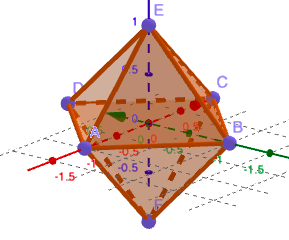
\includegraphics[width=0.4\textwidth]{L1.png}
            \caption{The $L^1$ unit ball in 3 dimensions}
            \label{fig:L1UB}
        \end{figure}
        \end{itemize}
        \end{frame}
        \begin{frame}{Monte Carlo Strategies: Simple Monte Carlo}
        \begin{itemize}
        \item Note that
        $$ \text{Vol}(B^{1}_{1}(0)) = \int_{B^{1}_{1}(0)}\,dx = 8\int_{[-1,1]^3}\chi_{B^{1}_{1}(0)}\frac{1}{8}\chi_{[-1,1]}\,dx$$
        \pause
        \item Sample $N$ points in the unit cube in 3 dimensions and if the sampled point lies in the unit ball, record that as a 1, and if not record it as a 0. In the end, add up all the 1's and divide by $N$. 
    \end{itemize}
\end{frame}

\begin{frame}{Monte Carlo Strategies: Simple Monte Carlo}
    \begin{figure}
        \centering
        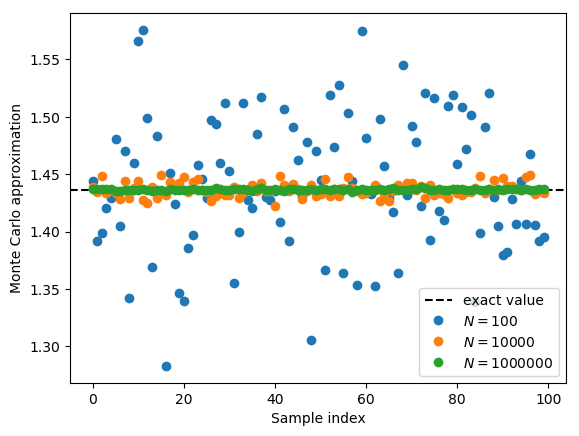
\includegraphics[width=0.7\textwidth]{output_11_0.png}
        \caption{Computing $\text{Vol}(B^{1}_{1}(0))$}
        \label{fig:SMC}
    \end{figure}
\end{frame}

\end{subsection}

\begin{subsection}{Importance Sampling}
\begin{frame}{Monte Carlo Strategies: Importance Sampling}
    \begin{itemize}
        \item Note that the $N=100$ case is particularly bad for SMC. 
        \pause
        \item This is because 
        $$ Var(\langle f \rangle) = \frac{\text{Var}(f(X))}{N} \approx \mathcal{O}(N^{-1})$$
       the variance of the estimator depends on the variance of the underlying distribution $X$, which is uniform in SMC. \pause
        \item Tweaking the distribution of $X$ might improve the variance of the estimator and hence the accuracy of our results. 
        \pause
        \item This is termed \textbf{Importance Sampling}
    \end{itemize}
\end{frame}

\begin{frame}{Monte Carlo Strategies: Importance Sampling}
\begin{itemize}
    \item Let's compute 
\[ I = \int_{[0,1]}2(1-x)e^x\,dx\]
\pause
\item SMC: $f(x) = 2(1-x)e^x$ and $\mu(x) = \chi_{[0,1]}$.
\pause
\item Importance Sampling: $f(x) = e^x$ and $\mu(x) = 2(1-x)$
\pause
\item In the importance sampling case, the points will be sampled with a density of $2(1-x)$. 
\end{itemize}
\end{frame}

\begin{frame}{Monte Carlo Strategies: Importance Sampling}
    \begin{figure}
        \centering
        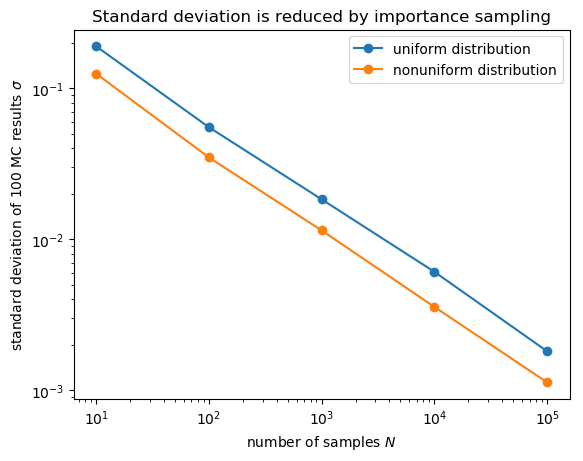
\includegraphics[width=0.7\textwidth]{output_16_0.png}
        \caption{Importance Sampling improves accuracy!}
        \label{fig:IS vs SMC}
    \end{figure}
\end{frame}
\end{subsection}

\begin{subsection}{Recursive Stratified Sampling}
\begin{frame}{Monte Carlo Strategies: Recursive Stratified Sampling}
    \begin{itemize}
    \item Although IS improved the variance, the rate of convergence remained $1/N$. 
    \pause
    \item \textbf{Recursive Stratified Sampling} helps this problem. 
    \pause
    \item We divide the domain of integration, $D$ into subdomains of equal size, termed $A$ and $B$ and compute $I$ in the following way:
    \pause
    \begin{figure}
        \centering
        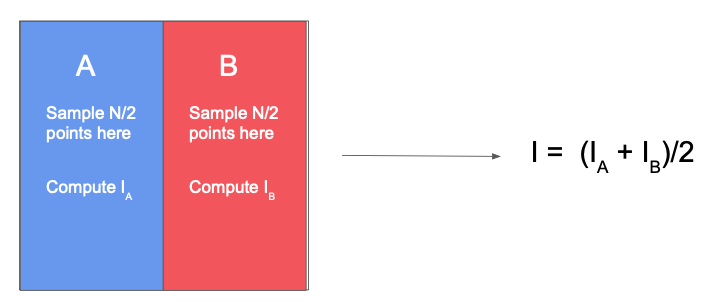
\includegraphics[width=0.7\textwidth]{RSS.png}
        \caption{How RSS works}
        \label{fig:HowRSSworks}
    \end{figure}
    \end{itemize}
    \end{frame}
    
    \begin{frame}{Recursive Stratified Sampling}
    \begin{itemize}
    \item That the estimator \(\langle f \rangle '\) can be viewed as a restricted case of the standard Monte Carlo estimator \(\langle f \rangle\) where half the points are sampled independently from \(A\) and the other half is sampled independently from \(B\):
    \pause
   $$I \approx \frac{1}{2}\Big(\frac{1}{N/2}\sum_{i=1}^{N/2}f_{A}(X_i) + \frac{1}{N/2}\sum_{i=1}^{N/2}f_{B}(X_i)\Big) = \langle f \rangle '$$
   \pause
   \item \textbf{Parallel Axis theorem}: $\sigma^2(\langle f \rangle) \geq \sigma^{2}(\langle f \rangle ')$
\end{itemize}
\end{frame}

\begin{frame}{Monte Carlo Strategies: Recursive Stratified Sampling}
    Compute $I$ by repeatedly subdividing $D$ and computing $\langle f \rangle '$ at each step. This is the $\textbf{Recursive Stratified Sampling}$ algorithm: 
    \pause
    \begin{figure}
        \centering
        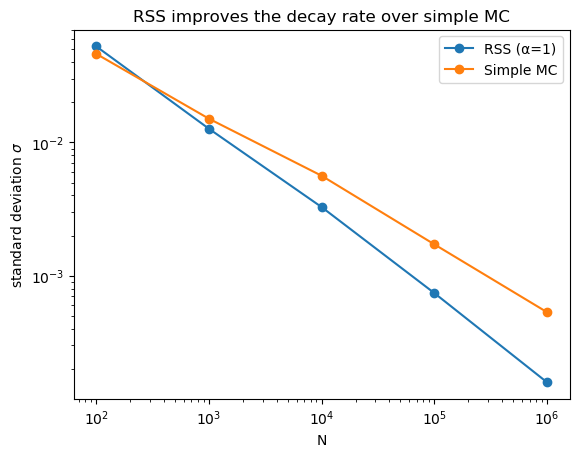
\includegraphics[width=0.65\textwidth]{output_22_0.png}
        \caption{RSS improves the rate of convergence!}
        \label{fig:RSS vs SMC}
    \end{figure}
\end{frame}
\end{subsection}

\begin{frame}{Monte Carlo algorithms: Summary}
    \begin{itemize}
        \item The SMC, IS, and RSS algorithms are all modifications of the Monte Carlo estimator. 
        \pause
        \item Importance sampling maintains the 1/2 rate of convergence, but improves the variance by a constant.
        \pause
        \item RSS improves the rate of convergence: it is more desirable method when the function is cheap to sample. 
        \pause
        \item Despite these improvements, we still need about 1 million function samples to get to within 4 digits of the true answer
        \pause
        \item The Bayesian estimator solves this accuracy problem dramatically.
    \end{itemize}
\end{frame}
\end{section}

\begin{section}{Bayesian Quadrature}

\begin{frame}{Bayesian Quadrature}
    \begin{itemize}
        \item The Bayesian strategy: $I$ is itself random and depends on the observed values of $f$.
        \pause
        \item There is inherent uncertainty in the value of $f(x)$. We need a prior on $f$ to our beliefs on the value of $f(x)$.  
        \pause
        \item Let $x_i$ be sampled independently from $X$ and let $\textbf{f} = [f(x_1) \ldots f(x_n)]^{\top}$ be the vector of observed values of $f$. Then obtain a posterior on $f$, (termed $\hat{f}$) by conditioning on $\textbf{f}$.
        \pause
        \item Next, compute $\hat{I} \mid \textbf{f}, \hat{f}$ where $\hat{I} = \int_{[0,1]}f(x)\mu(x)\,dx$. Note that $I$ is a function of the posterior distribution! 
        \pause
        \item Provided a convenient prior on $f$ we can use the expectation of $\hat{I}$ viewed as a distribution to estimate $I$. This is \textbf{Bayesian Quadrature}.
    \end{itemize}
\end{frame}

\begin{subsection}{Gaussian Processes}
\begin{frame}{Gaussian Processes: Motivation}
    \begin{itemize}
     \item A natural choice: $f(x) \sim N(m(x), \sigma(x))$
     \begin{figure}[h]
         \centering
         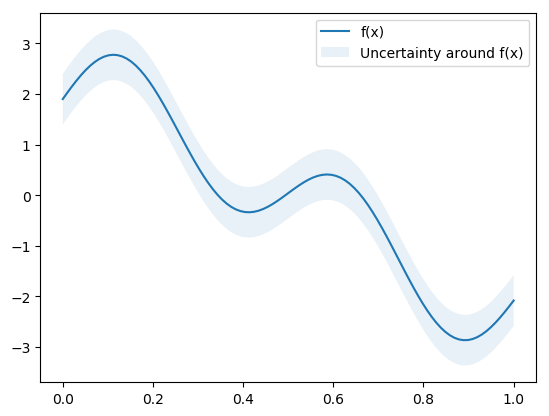
\includegraphics[width=0.66\textwidth]{output_24_0.png}
         \label{fig:GP}
     \end{figure}
    \end{itemize}
\end{frame}

\begin{frame}{Gaussian Processes: Definition}
    \begin{itemize}
        \item Let $GP$ be a distribution on functions $f: [0,1] \mapsto \mathbb{R}$. $GP$ is termed a \textbf{Gaussian Process} when for any finite set of points $D = [x_1, \ldots x_n]$, the finite set of values of $f$, i.e $f(D) = [f(x_1) \ldots f(x_n)]^{\top}$ follows a joint normal distribution with mean $\mu$ and covariance matrix $k(D,D)$. 
        \pause
        \item Furthermore, $\mu$ and $k(D,D)$ entries of $k(D,D)$, termed $k(x,x')$ are given by a function called a \textit{covariance kernel} satisfying symmetry, positivity, and 1-definiteness, i.e $k(x,x') = k(x',x)$, $k(x,y) > 0$, and $k(x,x) = 1$.
        \pause
        \item Note that if $D = \{x\}$ then $f \sim N(\mu(x), k(x,x))$
        % \item Note that if $D = \{x\}$, then we have that $f(x)$ is normally distributed with mean $\mu$ and a $1 \times 1$ covariance matrix, i.e variance $\sigma^2$ so Gaussian processes perfectly generalized the natural approach of putting a Gaussian prior around each value of $f$.  
    \end{itemize}
\end{frame}

\begin{frame}{Gaussian Processes: Example}
    \begin{figure}
        \centering
        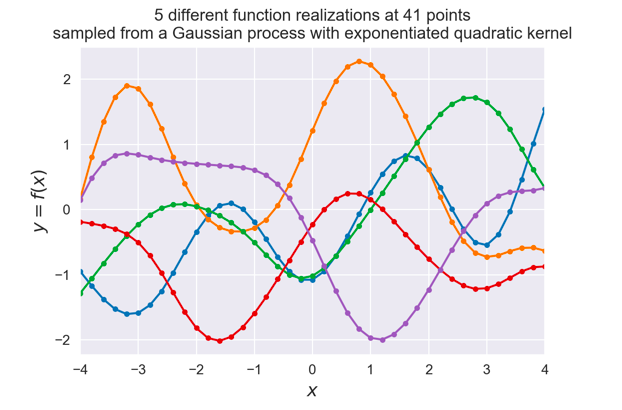
\includegraphics[width=0.9\textwidth]{GP1.png}
        \caption{Illustrating a Gaussian process (\cite{PR})}
        \label{fig:GP1}
    \end{figure}
\end{frame}
\begin{frame}{Gaussian Processes: Theoretical results}
    \begin{theorem}[\cite{PR}]
    Let $f \sim GP$ and $f(D)$ be a set of finite evaluations of $f$ on the set $D$. Then $f \mid \textbf{f} \sim GP$
    \end{theorem}
    
    This result follows from the fact that the conditional of a joint normal conditioned on any subset of the variables is also a joint normal.
    
    \begin{corollary}[\cite{minka2000}]
    Fix $x \in [0,1]$. Then 
    $$ f(x) \mid \textbf{f} \sim N(k(x,D)k(D,D)^{-1}f(D), k(x,x) - k(x,D)k(D,D)^{-1}k(D,x))$$
    \end{corollary}
     
     The above corollary gives an explicit formula for $f(x)$ as a posterior distribution. 
\end{frame}

\begin{frame}{Gaussian Processes: Theoretical Results (contd.)}

\begin{theorem}[Commutativity of Expectations (\cite{RG})]
Let $\Bar{f}$ be the posterior mean of $f \mid f(D)$. Then $$ \mathbb{E}_{f\mid f(D)}[\mathbb{E}_{X}[f\mid f(D)]] = \mathbb{E}_{X}[\Bar{f}]$$ 
\end{theorem}

\end{frame}
\end{subsection}

\begin{frame}{Gaussian Processes: The posterior process}
    \begin{figure}
        \centering
        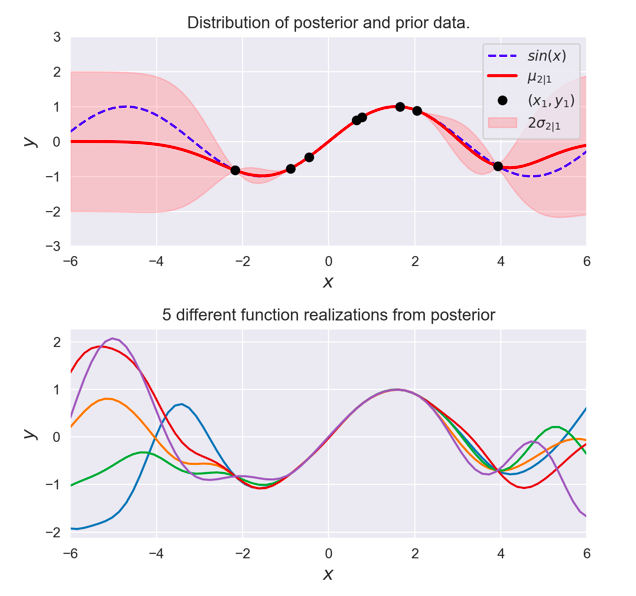
\includegraphics[width=0.7\textwidth]{GP2.png}
        \caption{Sharpening beliefs from sampling (\cite{PR})}
        \label{fig:GP2}
    \end{figure}
\end{frame}

\begin{subsection}{Algorithm}
\begin{frame}{A simple Bayesian quadrature algorithm}
    \begin{itemize}
        \item $I \approx \int_{[0,1]}m(x)\mu(x)\,dx$ where $$m(x) = k(x,D)k(D,D)^{-1}f(D)$$
        \pause
        \item Plugging in for $m$ we have that 
        \pause
        $$ \hat{I} = (u(D))^{\top}k(D,D)^{-1}f(D)$$
        
        where $(u(D))^{\top} = \int_{[0,1]}k(x,D)\mu(x)\,dx$
        \pause
        \item The variance of the estimator doesn't even depend on function values!
        \pause 
        \item However, to keep the algorithm probabilistic, we need not worry about variance minimzation. 
    \end{itemize}
\end{frame}

\begin{frame}{A Simple Bayesian quadrature algorithm}
    \begin{itemize}
        \item Let's compute $I = \int_{[0,1]}x^2\,dx$ using Bayesian Quadrature! 
        \pause
        \item Pick \(k\) to be the \(\textbf{Lorentzian Kernel}\), where 
        \[ k(x,y) = \frac{1}{1+|x-y|^2}\]
        \pause
        \item \((u(D))^{\top}\) can be computed analytically when \(\mu(x) \equiv 1\):
        
        \begin{align*}
            \int_{[0,1]}k(x,x_i)\mu(x)\,dx &= \int_{[0,1]}\frac{1}{1-|x-x_i|^2}\,dx \\ 
            &= \arctan(1-x_i) - \arctan(-x_i) \\
            &= \arctan(1-x_i) + \arctan(x_i)
            \end{align*}
    \end{itemize}
\end{frame}

\begin{frame}{A Simple Bayesian Quadrature algorithm}

    It takes only 10 samples for Bayesian Quadrature to get within 4 digits of the true answer while Monte Carlo will likely take more than 1000 samples. But BQ is also numerically unstable because it depends on inverting a matrix! 
    \begin{figure}[h]
        \centering
        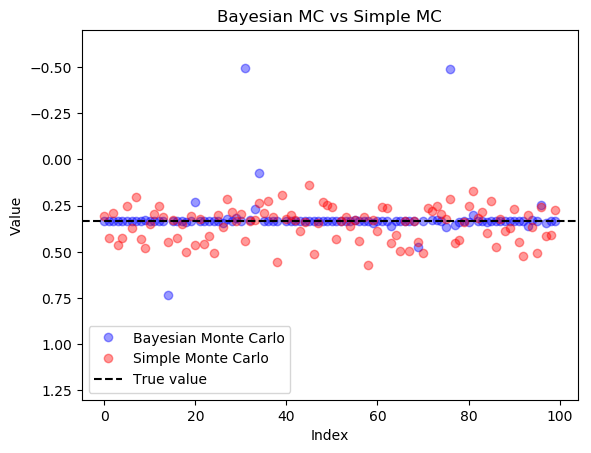
\includegraphics[width=0.6\textwidth]{output_30_0.png}
        \label{fig:Comparison}
    \end{figure}
    
    
\end{frame}
\end{subsection}
\end{section}
\begin{section}{Conclusion}

\begin{frame}{Conclusion}
\begin{itemize}
    \item Monte Carlo: numerically efficient and dimension-independent.
    \pause 
    \item The importance sampling and RSS algorithms are more accuracy-efficient implementations of the Monte Carlo estimator, yet not as accurate as Bayesian Quadrature.
    \pause
    \item But BQ suffers from the curse of dimensionality and poor conditioning.
    \pause
    \item Conclusion: There is no one algorithm that is best for all integrals!
    \pause
    \item Acknowledgements: The Monte Carlo algorithms (Implemented in C) can be found in (\cite{PTVF}).
\end{itemize}    
\end{frame}

\end{section}

\begin{frame}{References}
    \printbibliography
\end{frame}

\end{document}